\section*{III. Methods}
\addcontentsline{toc}{section}{III.\hspace{0.14in}Methods}
\hspace{0.25in}
To image the surface mode and collect data from our biosensor we first prepare the flowcell chamber with the correct substrate or liquid that acts as our reference point for measuring changes in optical properties. After the chamber is prepared we then turn on the beam and rotate it until the coupling angle is reached. Once that angle is reached a dark band representing the angular position of the surface mode will be captured by the CCD. This position occurs at a certain pixel along the horizontal axis of the CCD and serves as the control position of the surface mode.

\begin{wrapfigure}{L}{4in}
	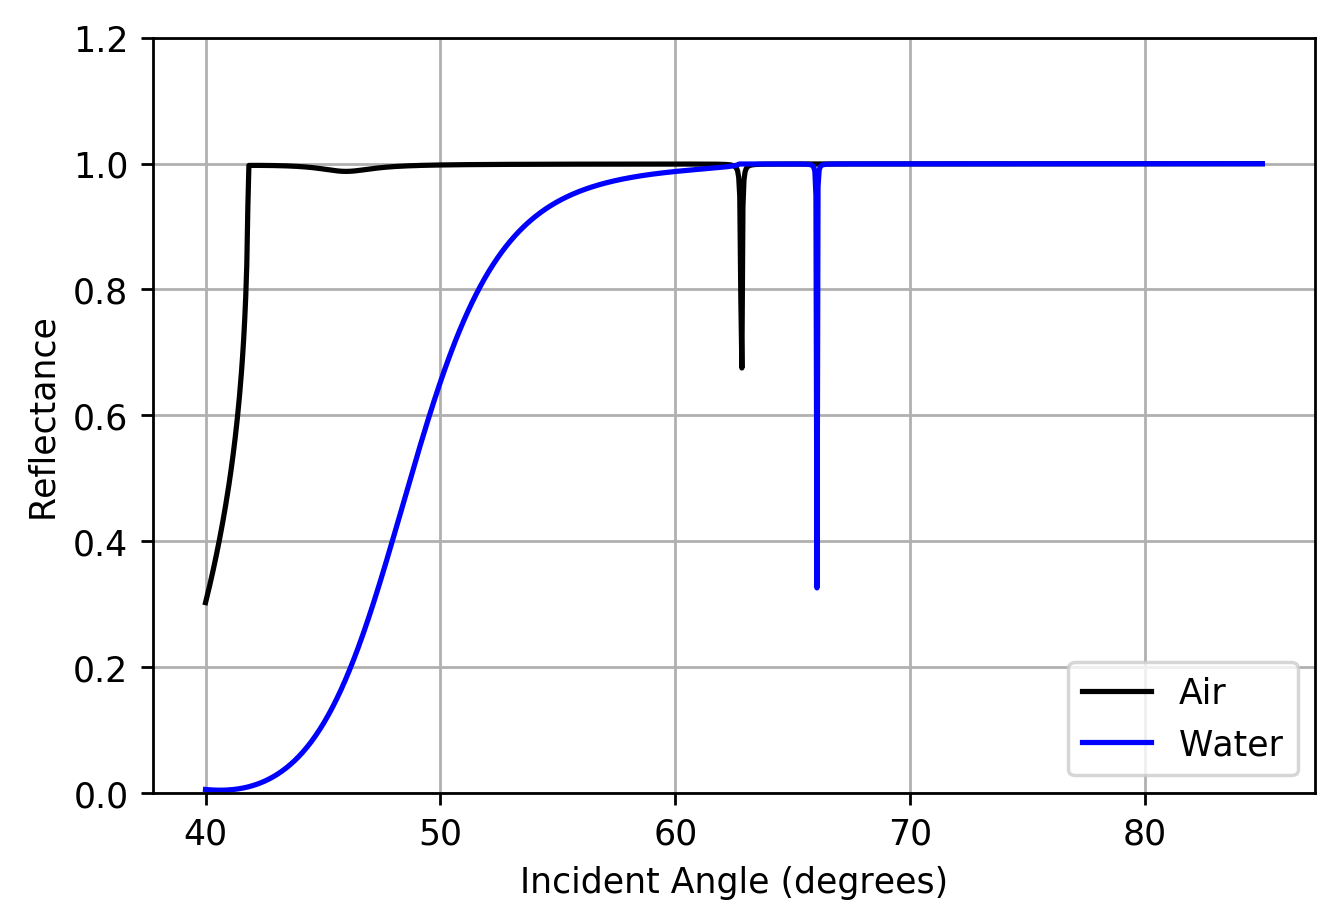
\includegraphics[width=4in]{reflectivity_dip.png}
	\caption{The reflectance characteristic of our multilayer. This plot was developed using a transfer matrix method.}
	\label{fig:reflectance}
\end{wrapfigure}

As the index of refraction inside the flowcell chamber changes the dark band will translate left or right from the control position of the surface mode in our reflected image, depending on whether the index is increasing or decreasing. The shift in location of the band, in pixels, corresponds to an angular shift in the part of the reflected beam giving rise to the dark band. This is shown clearly in \ref{fig:reflectance} as we see that a change from an index of 1.00 (air) to 1.33 (water) corresponds to an angular shift  of about $3^\circ$.


Using the calculated data we can build a model to relate the index of refraction in the chamber to a shift in pixels on our CCD. To construct this relation we require Snell's law and some geometry. Using the classic formula for arclength and the diagram below we find:\\

\begin{figure}[h!]
\begin{center}
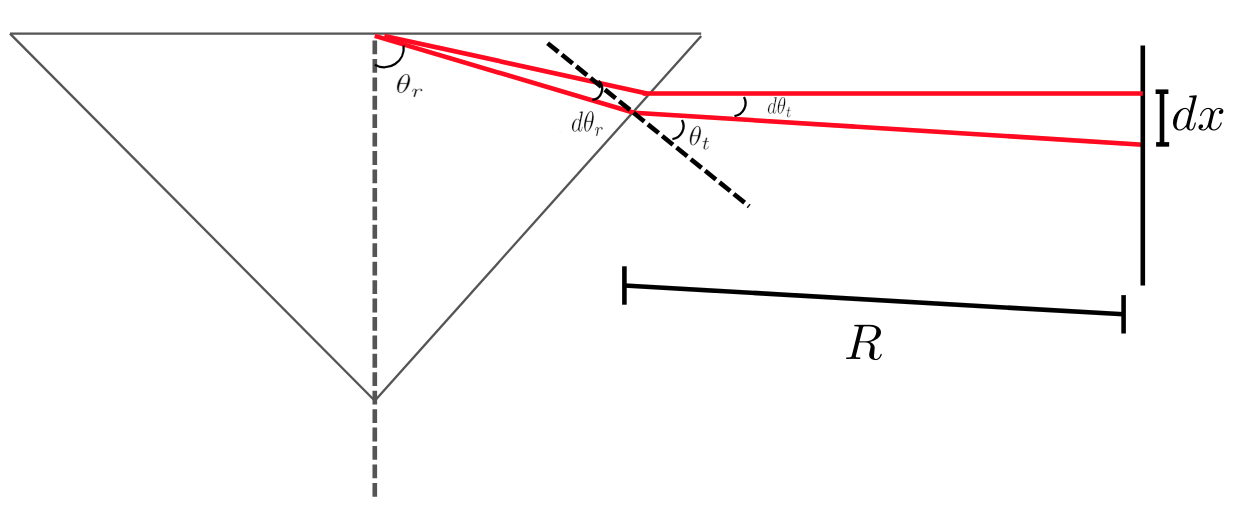
\includegraphics[width=0.8\textwidth]{pixelshiftfromangle.png}
\end{center}
\end{figure}

\begin{equation*}
	dx = R d\theta_t
\end{equation*}

Using Snell's law we find

\begin{equation*}
	\theta_t = \arcsin(\sin(n_g \theta_r))
\end{equation*}

Which implies that

\begin{equation*}
\begin{split}
	d\theta_t & = d\left(\arcsin\left(n_g \sin{\theta_r}\right)\right) \\
			  & = \cfrac{n_g \cos{\theta_r}}{\sqrt{1-n_g^2 \sin^{2}(\theta_r)}}\,\,d\theta_r
\end{split}
\end{equation*}

This leaves us with the relation between pixel shift and angular shift:

\begin{equation}
	dx = \cfrac{R n_g \cos{\theta_r}}{\sqrt{1-n_g^2 \sin^{2}(\theta_r)}} \,\,d\theta_r
\end{equation}

Numerically we can determine the relationship between the reflected angle and the index inside the chamber. I wrote a python program to do just that for our multilayer, assuming the chamber is initially filled with water, and a graph of mode position ($\theta_r$) vs index of refraction is plotted in Figure \ref{fig:modevsindex}.

\begin{figure}[h]
\begin{center}
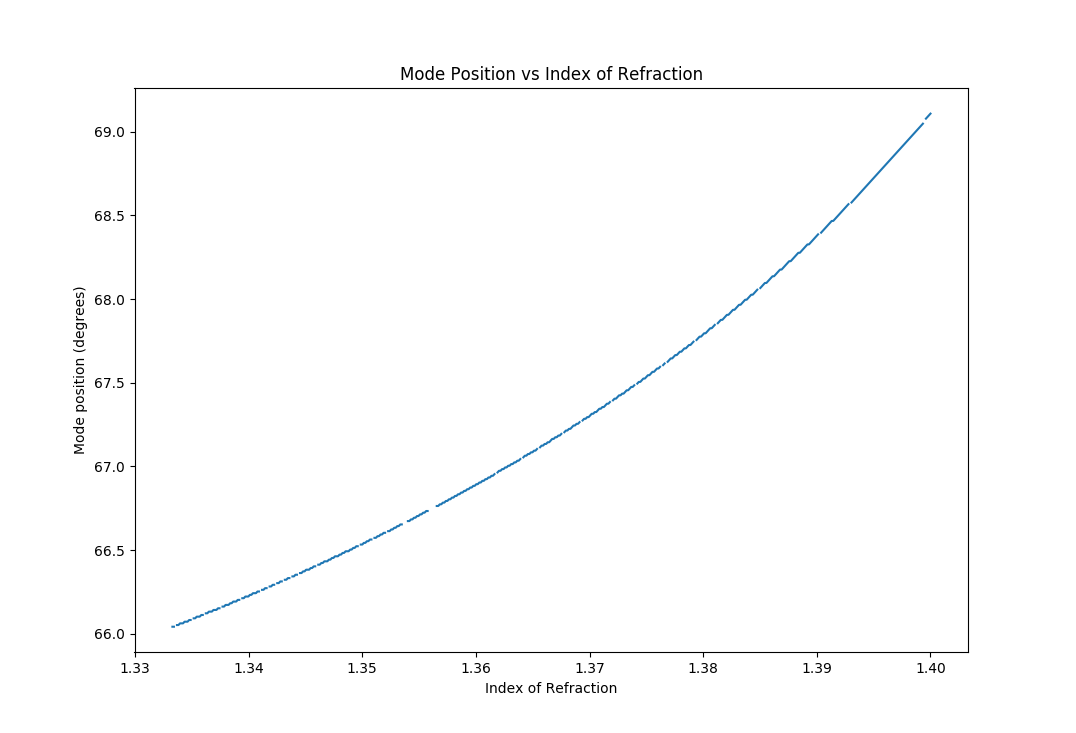
\includegraphics[width=\textwidth]{modeposition_vs_index.png}
\caption{The theoretical relation between the angular position of the mode and the index of refraction inside the flowcell chamber. }
\label{fig:modevsindex}
\end{center}
\end{figure}